\documentclass{article}
\usepackage{inputenc, amsmath, hyperref, amsfonts, graphicx, fancyhdr}

\title{Manifold Optimization Technical Note}
\author{Nathan Willey}
\date{July 2022}

\fancypagestyle{logo}{
\fancyhf{}
\fancyhead[LE,LO]{
\includegraphics[scale=.3]{../MTRI_logo.pdf}}}
\pagestyle{logo}

\begin{document}

\maketitle

\section*{Introduction}

This short technical note will detail the methods that the MATLAB package \href{www.manopt.org}{manOpt} uses for optimization over Riemannian manifolds. At the time of writing this is of particular interest over submanifolds of $\mathbb{R}^n$, but the methods used are valid on any Riemannian manifold. This note is meant to give a big-picture explanation of Riemannian gradients and their use in constrained optimization, omitting proofs and further details which can be found at the previous link or in the referenced texts. 

\section*{Method}

In this section I will give the basic knowledge leading to being able to solve an optimization problem over a (Riemannian) manifold with gradient descent.\\

For a function over a submanifold $\mathcal{M} \subset \mathbb{R}^n$, it is easy to compute the gradient $\nabla f(x)$. In an unconstrained optimization problem, $-\nabla f(x)$ gives the direction at x in which the function decreases the fastest. Here, however, there is no guarantee that $\nabla f$ points along the manifold, and thus a step in the direction of $-\nabla f(x)$ would violate the problem's manifold constraints. For this to be remedied we need to define the \textit{Riemannian Gradient} denoted $\text{grad}f(x) \in T_x \mathcal{M}$, the tangent space of $\mathcal{M}$ at x.\\

The Riemannian Gradient is defined to be the projection of $\nabla f$ onto $T_x \mathcal{M}$ using the endowed inner product of the manifold. This definition is well-defined and ensures the following relation:

\[D f(x)[v] = <v, \text{grad}f(x)>\]
Otherwise stated, for any path on the manifold at $x$ with "velocity" $v$, the directional derivative is equivalent to an inner product with the Riemannian gradient, exactly as in the Euclidean case. This definition also guarantees that moving on $\mathcal{M}$ in the direction of $-\text{grad}f(x)$ is again the direction of steepest descent.\\

Now for a gradient descent algorithm in a perfect world, we would like to follow along a geodesic on $\mathcal{M}$ aligned in the direction of $\text{grad}f(x)$. Computing geodesics, however, is very computationally expensive, and thus an inefficient way of proceeding.\\ Instead, we define a new mapping $\text{Retr}: (\mathcal{M}, \ T_x \mathcal{M}) \to \mathcal{M}$. This \textit{retraction} is what allows us to approximate movement along a geodesic at $x$ in the direction along a vector in the tangent space. As a simple example, (\ref{OptBlog}) gives a natural retraction on the unit sphere under an L-norm: $\text{Retr}(u, v)= \frac{u+v}{||u + v||_L}$, illustrated in [Figure \ref{sphere_retraction}].\\ With this final tool we are now able to compute the direction of steepest descent on a manifold $\text{grad}f(x)$ as well as approximate movement along the geodesic in that direction. 

\begin{figure}[h]
    \centering
    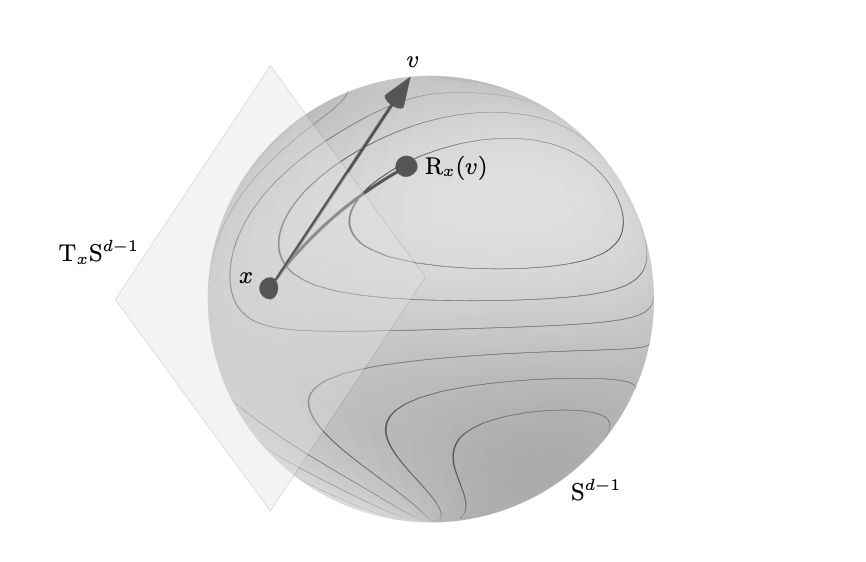
\includegraphics[width = 3in]{sphere_retraction.png}
    \caption{Movement along the unit sphere at $x$ in the direction of $v$ using the retraction $\text{Retr}(u, v)= \frac{u+v}{||u + v||_L}$. Figure taken from \ref{OptSmoothManifolds} (Figure 3.1)}
    \label{sphere_retraction}
\end{figure}

It is now natural to defined the method of gradient descent as 

\[x_{k+1} = \text{Retr}(x, -\alpha \text{grad}f(x))\]

where $\alpha$ can be determined through traditional line-search methods using the above formulation. \\
The retraction mapping used to approximate movement on the manifold is a \textit{choice} given by the user and different mappings may be better suited for varying objective functions. In this way, these methods for manifold optimization still require a choice on how to move along the manifold from free Euclidean space, though they perform the steps arguably more directly on the manifold without any necessary reparametrization of the input-space.\\

As an aside for this note, it is possible to compute a Riemannian Hessian using the same ideas of projecting the gradient onto the tangent space of a manifold. Through this, analogs for trust-region and bfgs methods have been created for Riemannian manifolds and are included in manOpt and described in more detail in \ref{OptSmoothManifolds}.





\begin{thebibliography}{9}

\bibitem{OptMatrixManifolds}
    \label{OptMatrixManifolds}
  P.-A. Absil, R. Mahoney, and Rodolphe Sepulchre,
  \textit{Optimization Algorithms on Matrix Manifolds},
  2008
  
\bibitem{OptSmoothManifolds}
    \label{OptSmoothManifolds}
    Nicolas Boumal,
    \textit{An Introduction to Optimization on Smooth Manifolds},
    2020

\bibitem{OptBlog}
    \label{OptBlog}
    Nicolas Boumal,
    \textit{Optimizing in smooth waters: optimization on manifolds},
    2015

\end{thebibliography}

\end{document}
